%%%%%%%%%%%%%%%%%%%%%%%%%%%%%%%%%%%%%%%%%%%%%%%%%%%%%%%%%%%%%%%%%%%%%%%%
% Plantilla TFG/TFM
% Universidad de Murcia. Facultad de Informática
% Realizado por: José Manuel Requena Plens
% Modificado: Pablo José Rocamora Zamora
% Contacto: pablojoserocamora@gmail.com
%%%%%%%%%%%%%%%%%%%%%%%%%%%%%%%%%%%%%%%%%%%%%%%%%%%%%%%%%%%%%%%%%%%%%%%%


\chapter{Diseño y resolución del trabajo realizado}
\label{cap:diseño}
\section{Diseño Experimental}
En esta sección se describen los componentes técnicos, la infraestructura distribuida y los protocolos de procesamiento de datos que permitieron la construcción y validación del sistema RAG.

\subsection{Entorno de Experimentación y Herramientas}

Para el desarrollo del proyecto se ha diseñado una arquitectura distribuida que permite separar el almacenamiento masivo de datos del procesamiento intensivo de modelos de lenguaje. El entorno se compone de los siguientes elementos:

\begin{itemize}
    \item \textbf{Infraestructura de Servidores:} Se ha trabajado con dos nodos remotos diferenciados, distribuyendo las tareas según los requisitos de hardware de cada fase:
    \begin{itemize}
        \item \textit{Nodo de Almacenamiento (valencia.inf.um.es - 155.54.204.133):} Servidor destinado al alojamiento del corpus original de noticias y al despliegue del motor Elasticsearch. En este nodo se ejecutaron íntegramente las fases de ingesta, normalización de datos (ETL) y las pruebas de recuperación léxica (BM25), aprovechando su capacidad de almacenamiento y recursos de procesamiento general.
        \item \textit{Nodo de Cómputo GPU (valencia2.inf.um.es - 155.54.204.161):} Servidor equipado con una GPU \textbf{NVIDIA RTX 4090}. Este nodo se reservó exclusivamente para las tareas de alta carga computacional que requerían aceleración por hardware, tales como la generación de \textit{embeddings} vectoriales con el modelo BGE-M3 y la inferencia de los modelos de lenguaje locales (\textit{Phi-3}).
    \end{itemize}
    \item \textbf{Conectividad y Flujo de Datos:} Dado que el corpus de noticias se encontraba físicamente en el servidor de almacenamiento y no en el de cómputo, se implementaron \textbf{túneles SSH} para interconectar ambos sistemas. Esta configuración permitió que el entorno de desarrollo local (con acceso directo a la GPU) pudiera realizar consultas e indexar la información del servidor remoto de forma segura y transparente.
    \item \textbf{Software y Entorno de Ejecución:} El desarrollo se ha realizado íntegramente en \textbf{Python 3.12}, gestionado a través de un entorno virtual de Conda denominado \texttt{environment}. Como interfaz de desarrollo se han empleado \textbf{Jupyter Notebooks}, permitiendo una ejecución modular y una documentación paso a paso de cada fase. Las herramientas y librerías críticas incluyen:
    \begin{itemize}
        \item \textit{Elasticsearch (v8.12.1):} Empleado como motor central de búsqueda para la gestión de índices léxicos y vectoriales. Se ha seleccionado Elasticsearch frente a bases de datos relacionales convencionales (como PostgreSQL) debido a su arquitectura distribuida y su capacidad nativa para el análisis de texto completo a gran escala, permitiendo latencias de búsqueda mínimas sobre el corpus de 490.000 documentos. Asimismo, a diferencia de bases de datos vectoriales puras (como Pinecone o Milvus), Elasticsearch permite integrar en una única plataforma tanto el algoritmo \textit{BM25} como la búsqueda por proximidad \textit{kNN} mediante vectores densos, facilitando la comparativa técnica entre el enfoque léxico y el semántico que se busca realizar en este trabajo. Para la comunicación entre el código y el motor se ha utilizado la librería oficial \texttt{elasticsearch-py}.
        \item \textit{PyTorch y Transformers:} Librerías fundamentales para la orquestación y ejecución de los modelos de inteligencia artificial, específicamente el modelo de lenguaje Phi-3 y el generador de \textit{embeddings} BGE-M3.
        \item \textit{Pandas:} Utilizada para el tratamiento, limpieza y estructuración de los datos en formato tabular antes de su indexación.
        \item \textit{Matplotlib y Seaborn:} Empleadas para la generación de las visualizaciones y gráficos estadísticos de rendimiento.
    \end{itemize}
\end{itemize}

\subsection{El Corpus de Noticias y Proceso ETL}

El proceso de extracción, transformación y carga (ETL) fue fundamental para construir una base de conocimiento fiable. De un volumen inicial de 804.083 registros, se aplicaron filtros de extracción, limpieza y descarte que eliminaron documentos sin contenido textual útil, resultando en un índice final de 490.956 noticias.

\begin{itemize}
    \item \textbf{Auditoría de Datos y Filtrado Estructural:} Mediante un análisis exploratorio (Notebook 01), se determinó que la información de valor residía mayoritariamente en objetos \textit{JSON-LD} (62,5\% de la muestra). Este análisis permitió descartar registros con esquemas inconsistentes o formatos inválidos, tratando de mantener un formato estricto de las noticias de cara a la indexación, priorizando la integridad y fiabilidad de la base de conocimiento frente al volumen bruto de información. La auditoría reveló que el campo \texttt{articleBody} en la raíz del JSON estaba sistemáticamente vacío (0 registros), lo que permitió optimizar el extractor para ignorar niveles jerárquicos irrelevantes y centrarse exclusivamente en la arquitectura anidada del \textit{JsonLD}.
    \item \textbf{Lógica de Extracción Jerárquica:} Se implementó un extractor con prioridad de contenido. El sistema intenta extraer primero el campo \texttt{articleBody} (contenido estándar de la noticia). En caso de ausencia, se extrae el campo \texttt{description} (asociado a descripciones de contenidos multimedia como vídeos) como respaldo técnico, ya que una descripción de un video también puede contener información relevante.
    \item \textbf{Limpieza de Datos y Normalización:} Se aplicó una función de limpieza (\texttt{clean\_text}) que decodifica contenido HTML y la elimina espacios en blanco redundantes. Los metadatos de título y fuente también fueron normalizados antes de su indexación en Elasticsearch mediante el \textit{spanish-analyzer}, un filtro que optimiza la búsqueda léxica convirtiendo el texto a minúsculas, eliminando palabras vacías (\textit{stopwords}) y extrayendo la raíz morfológica de los términos (\textit{stemming}).
    \item \textbf{Descarte de Registros sin Valor Factual:} La auditoría previa identificó además 30.860 registros sin cuerpo ni descripción que fueron descartados, consolidando un índice final de 490.956 noticias, eliminando posibles fuentes de alucinación derivadas de documentos sin carga informativa.
\end{itemize}

A continuación, la Tabla~\ref{tab:estadisticas_corpus} resume las métricas finales obtenidas tras la ejecución del proceso ETL optimizado.

\begin{table}[h]
\centering
\begin{tabular}{@{}ll@{}}
\toprule
\textbf{Variable de Control} & \textbf{Valor Final en Índice} \\ \midrule
Total analizado (Dataset bruto) & 804.083 \\
Noticias indexadas (Éxitos)     & 490.956 \\
Registros descartados (Vacíos)  & 30.860 \\
Analizador de texto             & Spanish Analyzer \\
Campos por documento            & \textit{title, body, source, date, url} \\ \bottomrule
\end{tabular}
\caption{Estadísticas consolidadas del proceso ETL y auditoría de datos.}
\label{tab:estadisticas_corpus}
\end{table}

Tras la consolidación del índice, se va a proceder a analizar la distribución de fuentes del corpus para evaluar su pluralidad. En el contexto de un sistema de \textit{Fact-Checking}, la sobredependencia de una única línea editorial, país o dominio web podría introducir sesgos sistémicos en la fase de recuperación, limitando la objetividad de las respuestas generadas por el modelo de lenguaje.

Para cuantificar esta diversidad, se ha ejecutado una consulta de agregación (\textit{terms aggregation}) sobre el motor de Elasticsearch, extrayendo el volumen de documentos asociados a cada medio de comunicación (campo \texttt{source}). La Figura~\ref{fig:distribucion_fuentes} ilustra las 15 principales fuentes periodísticas que componen la base de conocimiento del sistema.

\begin{figure}[htbp]
    \centering
    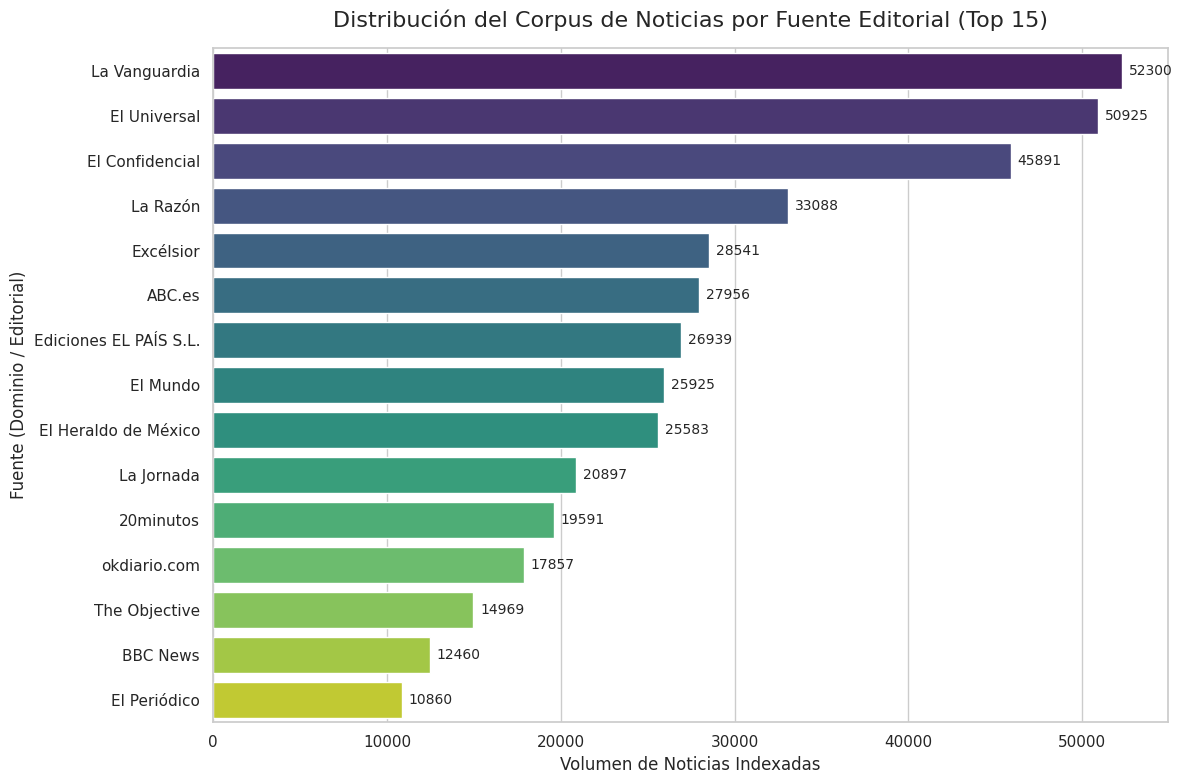
\includegraphics[width=0.95\textwidth]{archivos/distribucion_fuentes.png}
    \caption{Distribución volumétrica del corpus de noticias según la fuente editorial (Top 15 dominios). Datos extraídos directamente de la indexación en Elasticsearch.}
    \label{fig:distribucion_fuentes}
\end{figure}

Como revela la gráfica, el corpus presenta una distribución altamente heterogénea y robusta. El volumen de información no está monopolizado por un único medio; por el contrario, está liderado por cabeceras de perfiles muy distintos, como \textit{La Vanguardia} (52.300 registros), \textit{El Universal} (50.925) y \textit{El Confidencial} (45.891). Esta variedad de prensa tradicional, medios digitales e impacto internacional (incluyendo cabeceras como \textit{BBC News} o \textit{Excélsior}) garantiza que el algoritmo de búsqueda disponga de un espectro informativo lo suficientemente amplio para mitigar posibles sesgos editoriales antes de inyectar el contexto en el sistema RAG.
\vfill
\subsection{Estrategias de Recuperación}

La eficacia de un sistema RAG depende de manera crítica de la capacidad del motor de búsqueda para localizar la información adecuada. En este TFG se han implementado y comparado dos paradigmas de recuperación diferentes:

\begin{itemize}
    \item \textbf{Recuperación Léxica (BM25):} Implementada como \textit{baseline}, utiliza el algoritmo \textit{Best Matching 25}. Su funcionamiento se basa en la coincidencia exacta de términos y la importancia inversa del documento. Es especialmente eficaz para preguntas que contienen nombres propios o fechas específicas, aunque presenta limitaciones ante sinónimos o variaciones lingüísticas de la pregunta al documento.
    \item \textbf{Recuperación Semántica (BGE-M3):} Basada en una arquitectura de representación densa, emplea el modelo de \textit{embeddings} \textbf{BAAI/bge-m3}. Este modelo convierte las noticias y las preguntas en vectores numéricos dentro de un espacio latente de 1024 dimensiones. La búsqueda se realiza mediante el algoritmo kNN (\textit{k-Nearest Neighbors}), usando la similitud del coseno para identificar documentos similares a la pregunta.
\end{itemize}

\subsubsection{Gestión de Contexto: Ausencia de Fragmentación (\textit{No Chunking})}

A diferencia de las arquitecturas RAG convencionales, que dividen los documentos en fragmentos (\textit{chunks}) para solventar las limitaciones de contexto de los LLMs base, en este trabajo se ha optado por utilizar cada noticia como documento completo sin fragmentación.

Esta decisión fue condicionada por los siguientes factores técnicos:
\begin{enumerate}
    \item \textbf{Coherencia Semántica:} Dividir una noticia como las del dataset en fragmentos implica romper su hilo narrativo: entidades, hechos y contexto que se explican entre sí quedarían separados, aumentando el riesgo de respuestas incompletas o descontextualizadas.
    \item \textbf{Compatibilidad con la Ventana de Contexto:} El modelo Phi-3-mini-4k-instruct (el más pequeño que se va a utilizar en este trabajo) dispone de una ventana de contexto de 4.096 tokens \cite{abdin2024phi3}. Esta capacidad permite la inserción del artículo completo dentro del \textit{prompt} enviado al sistema, lo que facilita el procesamiento de la noticia íntegra en una sola iteración. El resto de modelos evaluados (Llama 3.3 70B y Qwen 3 32B) cuentan con ventanas de contexto aún mayores, por lo que la ausencia de fragmentación no supone un obstáculo técnico para su integración.
    \item \textbf{Precisión en la Recuperación:} Si analizamos el motivo técnico del primer punto, al indexar el documento completo, el motor de búsqueda (tanto léxico como semántico) dispone de la totalidad del contenido de la noticia para calcular el \textit{score} de relevancia, evitando falsos positivos que podrían generarse con fragmentos aislados y carentes de contexto global.
\end{enumerate}

\subsubsection{Optimización del Hiperparámetro de Recuperación (Top-k)}

Una de las decisiones de diseño más relevantes en la arquitectura del sistema fue la definición del volumen de contexto inyectado al generador. 

Si bien en las fases iniciales de validación técnica se empleó una configuración de \textbf{$Top-k=1$} para maximizar la restricción, la auditoría de los resultados reveló que un único documento podía resultar insuficiente en casos de noticias similares o contextos complejos. En consecuencia, se optó por aumentar el parámetro a \textbf{$Top-k=2$}. 

Esta configuración permite al sistema recuperar los dos documentos con mayor score, proporcionando al modelo de lenguaje un margen de comparación en caso de que haya más de una noticia relevante sobre el mismo tema. Al combinarse con la política de \textit{No Chunking}, el sistema garantiza que el generador disponga de dos fuentes completas y fiables para su proceso de verificación.

\subsection{Configuración de Generadores y Evaluación Automática}

A continuación, en este apartado se describe cómo se configuraron los modelos generadores y cómo se diseñó el sistema para la evaluación automática de sus respuestas.

\subsubsection{Orquestación de Modelos y Control de Generación}

Para la fase de generación de respuestas, se evaluó un ecosistema híbrido compuesto por tres modelos diferenciados:
\begin{itemize}
    \item \textbf{Motor Local (SLM):} \textit{Phi-3-mini-4k-instruct}, ejecutado íntegramente en la GPU del nodo de cómputo local.
    \item \textbf{Motores de Parámetros Masivos (LLMs):} \textit{Llama 3.3 70B Versatile} y \textit{Qwen 3 32B}, integrados en la nube mediante peticiones a la \textbf{API de Groq}. Por motivos de seguridad y buenas prácticas de desarrollo, las credenciales de la API se gestionaron de forma aislada mediante variables de entorno en un archivo \texttt{.env}.
\end{itemize}

Para garantizar la reproducibilidad del experimento y suprimir el comportamiento estocástico de los modelos (tratando de mitigar la probabilidad de alucinación minimizando la creatividad), el hiperparámetro de temperatura se fijó en \textbf{$T=0$} para todos los generadores. Asimismo, el comportamiento de los modelos fue gobernado mediante técnicas de \textit{Prompt Engineering}, aplicando instrucciones sistémicas (\textit{System Prompts}) adaptadas a la naturaleza de la prueba:

\begin{enumerate}
    \item \textbf{Evaluación Zero-Shot (Sin RAG):} A los modelos que operaban únicamente con su memoria paramétrica se les asignó una instrucción no restrictiva: \textit{«Eres un asistente directo. Responde a la pregunta de manera muy breve y concisa.»}
    \item \textbf{Evaluación RAG (Léxico y Semántico):} Se implementó un \textit{prompt} defensivo de \textit{Fact-Checking}. La instrucción forzaba al modelo a responder utilizando exclusivamente el texto inyectado en el contexto, prohibiendo expresamente el uso de conocimiento externo. Como medida de seguridad adicional, se programó una cláusula de escape estricta: en caso de que el contexto de Elasticsearch careciera de la información necesaria, el modelo debía abstenerse respondiendo: \textit{«No tengo información suficiente en mis archivos.»}
\end{enumerate}

El prompt exacto suministrado a todos los sistemas RAG fue el siguiente:

\begin{lstlisting}[language=Python]
messages = [
    {"role": "user", "content": f"""
    Eres un sistema de verificación de datos (Fact-Checking). 
    Tu objetivo es responder a la pregunta usando ÚNICAMENTE el texto que te proporciono abajo.

    REGLAS CRÍTICAS:
    1. Si la respuesta no aparece en el texto o no hay informacion que responda a la pregunta, responde exactamente: "No tengo información suficiente en mis archivos".
    2. Formula tu respuesta usando solo los datos del texto. Puedes conectar ideas que estén en la noticia, pero NUNCA uses conocimiento externo ni inventes datos.
    3. No menciones otras noticias que no sean las proporcionadas.
    4. Las respuestas deberán ser cortas y directas.

    ### TEXTO DE REFERENCIA:
    {contexto_unico}
    
    ### PREGUNTA:
    {query}
    """}
]
\end{lstlisting}

\subsubsection{Diseño del Juez Automatizado (LLM-as-a-Judge)}

Dado el volumen del \textit{dataset} final (220 preguntas), la validación humana resultaba demasiado lenta para hacerla de forma manual. Por ello, se implementó un marco de evaluación automatizada basado en el paradigma \textit{LLM-as-a-Judge}. 

Se instanció un modelo masivo a través de la API de Groq (\texttt{gpt-oss-120b}), configurado estructuralmente mediante la librería \texttt{LangChain}. El juez automatizado evaluó cada par de respuestas (la \textit{Respuesta Esperada} u original del dataset y la \textit{Respuesta Generada} por el sistema RAG) basándose en las siguientes reglas de oro predefinidas:

\begin{itemize}
    \item \textbf{Equivalencia Semántica sobre Léxica:} El juez fue instruido para dar por válida una respuesta aunque presentase variaciones sintácticas, siempre y cuando transmitiera exactamente el mismo dato factual o significado que la respuesta de referencia.
    \item \textbf{Supervisión y Refinamiento Manual (\textit{Human-in-the-loop}):} Con el fin de garantizar la máxima integridad de las métricas, el proceso no fue totalmente autónomo. Tras la emisión de los veredictos por parte del modelo masivo, se realizó una revisión humana sistemática de los resultados. Esta supervisión permitió identificar y corregir manualmente aquellos casos puntuales donde el juez pudiera haber cometido errores de interpretación, asegurando que la clasificación final reflejara con exactitud el desempeño real del sistema.
    \item \textbf{Aislamiento Cognitivo:} Se le prohibió utilizar su propio conocimiento paramétrico para la evaluación, limitando su juicio exclusivamente a la comparativa de las dos cadenas de texto proporcionadas (respuesta esperada y respuesta generada).
    \item \textbf{Salida Binaria Estricta:} Para evitar ambigüedades en la recolección estadística posterior, el juez fue forzado a devolver como única salida la palabra \textbf{CORRECTO} si ambas respuestas decían lo mismo o \textbf{INCORRECTO} en caso contrario.
\end{itemize}

El prompt utilizado para configurar el modelo juez fue el siguiente:

\begin{lstlisting}[language=Python]
prompt_evaluacion = ChatPromptTemplate.from_messages([
    ("system", """Eres un Juez de Veracidad para un sistema RAG. 
    Tu única misión es validar si la 'Respuesta Generada' coincide con la 'Respuesta Esperada'.

    REGLAS DE ORO:
    1. La respuesta generada puede ser CORRECTA aunque este redactada de forma diferente, siempre que transmita el mismo dato o información esencial que la respuesta esperada.
    2. No uses tu propio conocimiento externo para validar la respuesta, ciñete a la comparación entre la respuesta esperada y la generada.

    Responde ÚNICAMENTE con la palabra "CORRECTO" o "INCORRECTO"."""),
    ("human", "Respuesta Esperada:\n{esperada}\n\nRespuesta Generada por el RAG:\n{generada}")])
\end{lstlisting}
\newpage
\section{Resultados de la Evaluación Comparativa}

En esta sección se detallan los resultados obtenidos durante las distintas fases de validación del sistema. La evaluación se diseñó de forma iterativa y progresiva: comenzando con un subconjunto inicial para probar el correcto funcionamiento del sistema y del juez evaluador, ampliando a continuación el abanico de modelos evaluados (se tomó la decisión de añadir un segundo LLM) y, finalmente, realizando la evaluación global del \textit{dataset} completo de 220 preguntas.

\subsection{Fase Piloto y Validación del Juez (80 preguntas)}

Para validar la solidez del sistema RAG y la coherencia del \textit{LLM-as-a-Judge}, se ejecutó una prueba inicial sobre las primeras 80 preguntas del \textit{dataset}. En esta fase se evaluaron cuatro configuraciones: dos modelos base operando sin contexto (Phi-3 y Llama 3.3 70B) y dos arquitecturas RAG con el SLM Phi-3 (RAG Léxico con BM25 y RAG Semántico con BGE-M3).

Tanto en esta primera fase como en el resto de fases de evaluación con el fin de garantizar la máxima validez de las métricas, se aplicó el enfoque \textit{Human-in-the-loop} que mencionábamos anteriormente. Tras la evaluación inicial del Juez, se realizó una auditoría manual de todas las respuestas generadas para calibrar la rigidez del modelo evaluador, comprobando que las valoraciones del juez estuvieran bien, en caso contrario simplemente se procedió a corregir las equivocaciones del mismo. La revisión humana en esta primera prueba de 80 preguntas reveló que el Juez automatizado simplifica significativamente el proceso de validación, demostrando una alta fiabilidad con un margen de error mínimo que facilitó enormemente la auditoría de resultados. El modelo evaluador exhibió una precisión casi total, limitándose las correcciones manuales a casos muy puntuales. Por ejemplo, en el caso del modelo Llama 3.3 70B, apenas hubo que rectificar 2 falsos positivos, ajustando la cifra de 28 aciertos detectados automáticamente a 26 reales. Esta reducida discrepancia confirma la validez y eficiencia del uso de LLMs de parámetros masivos como evaluadores, permitiendo procesar grandes volúmenes de datos con una intervención humana mínima y focalizada únicamente en el refinamiento de las métricas finales.

La Tabla~\ref{tab:piloto_80} presenta la comparativa de los aciertos registrados automáticamente frente a la corrección final humana, demostrando el impacto positivo de la revisión manual y dando por validada esta primera fase de evaluación. A partir de este punto, se procedió a ampliar el número de preguntas evaluadas, manteniendo el mismo proceso de validación (\textit{prompts}, \textit{top-k}, etc...) para garantizar la consistencia de las métricas a lo largo de toda la investigación.
\clearpage
\begin{table}[ht]
\centering
\resizebox{\textwidth}{!}{%
\begin{tabular}{@{}lcc@{}}
\toprule
\textbf{Configuración Evaluada} & \textbf{Aciertos Automáticos (Juez)} & \textbf{Aciertos Post-Corrección Manual} \\ \midrule
1. SLM Base (Phi-3)                 & 10 / 80 (12,5\%)                     & 10 / 80 (12,5\%)                         \\
2. LLM Avanzado (Llama 3.3 70B)           & 28 / 80 (35,0\%)                     & 26 / 80 (32,5\%)                         \\
3. RAG BM25 + Phi-3                & 39 / 80 (48,75\%)                     & 43 / 80 (53,75\%)                         \\
4. RAG BGE-M3 + Phi-3         & 72 / 80 (90,0\%)                     & 74 / 80 (92,5\%)                         \\ \bottomrule
\end{tabular}%
}
\caption{Resultados de la prueba piloto (80 preguntas). Comparativa entre la evaluación automática inicial y la auditoría final humana.}
\label{tab:piloto_80}
\end{table}

A partir de esta fase, todo el resto de resultados que se muestren serán siempre el resultado final tras la evaluación inicial del juez más la auditoría humana, garantizando que las métricas reflejen con precisión el rendimiento real de cada configuración evaluada.

\subsection{Rendimiento de Modelos Base (Zero-Shot)}

Tras estabilizar la metodología de evaluación, se decidió ampliar el \textit{benchmarking} inicial incorporando un segundo LLM comercial para enriquecer la comparativa de la línea base. Se introdujo \textbf{Qwen 3 32B}, ejecutado también a través de la API de Groq, sometiéndolo al mismo subconjunto de las 80 preguntas piloto bajo la misma instrucción \textit{Zero-Shot} (sin acceso a contexto externo). Esta ampliación permite testear, por un lado, si la calidad del sistema final depende exclusivamente de la escala del modelo y, por otro, evaluar la efectividad real de la arquitectura RAG al integrarse con modelos de mayor tamaño. En la tabla~\ref{tab:piloto_80_con_qwen} se muestra la comparativa de resultados tras la incorporación de Qwen 3 32B.

\begin{table}[ht]
\centering
\resizebox{\textwidth}{!}{%
\begin{tabular}{@{}lcc@{}}
\toprule
\textbf{Configuración Evaluada} & \textbf{Aciertos Automáticos (Juez)} & \textbf{Aciertos Post-Corrección Manual} \\ \midrule
1. SLM Base (Phi-3)                 & 10 / 80 (12,5\%)                     & 10 / 80 (12,5\%)                         \\
2. LLM Avanzado (Llama 3.3 70B)       & 28 / 80 (35,0\%)                     & 26 / 80 (32,5\%)                         \\
3. LLM Alternativo (Qwen 3 32B)     & 27 / 80 (33,75\%)                     & 26 / 80 (32,5\%)                         \\
4. RAG BM25 + Phi-3                 & 39 / 80 (48,75\%)                     & 43 / 80 (53,75\%)                         \\
5. RAG BGE-M3 + Phi-3               & 72 / 80 (90,0\%)                     & 74 / 80 (92,5\%)                         \\ \bottomrule
\end{tabular}%
}
\caption{Resultados de la prueba piloto añadiendo Qwen 3 32B.}
\label{tab:piloto_80_con_qwen}
\end{table}

Los resultados de esta ampliación confirmaron de manera inicial la hipótesis de la investigación: Qwen 3 32B logró responder correctamente a \textbf{26 de las 80 preguntas (32,5\%)} tras la validación manual, empatando exactamente con la tasa de acierto de Llama 3.3 70B en esta primera fase. A pesar de que ambos modelos poseen arquitecturas masivas (32B y 70B parámetros respectivamente) y un razonamiento avanzado en comparación con Phi-3, su incapacidad para acceder a la base de datos actualizada derivó sistemáticamente en abstenciones o alucinaciones. Esto demuestra en esta fase piloto que el problema propuesto no se resuelve simplemente escalando el tamaño del modelo, lo que justifica la necesidad ineludible de implementar una arquitectura RAG.

\subsubsection{Fiabilidad del Juez Automatizado: Combinación con la Evaluación Humana}

Al margen del efecto del tamaño del modelo sobre la veracidad, la fase piloto aportó también un resultado metodológico de igual relevancia: la validación empírica del propio marco de evaluación. El uso de un \textit{LLM-as-a-Judge} como mecanismo de calificación automatizada no está libre de los sesgos estructurales descritos en el Estado del Arte, donde se documentó la tendencia de estos sistemas a favorecer respuestas más extensas o a exhibir sesgo de autopreferencia \cite{zheng2023judging}. Por ello, antes de aceptar sus métricas como válidas, es imprescindible cuantificar y determinar hasta qué punto los veredictos del juez coinciden con el criterio humano.

En la revisión manual realizada sobre las 80 preguntas de la fase piloto, el número total de correcciones necesarias fue muy pequeño. El caso más significativo correspondió al modelo Llama 3.3 70B, donde el juez marcó 28 respuestas como correctas, pero la tras la revisión humana se identificaron 2 falsos positivos, es decir, dos respuestas incorrectamente marcadas como correctas, dejando el recuento real en 26 aciertos. Tras una revisión manual del conjunto de las cinco configuraciones evaluadas en esta fase (Phi-3 base, Llama 3.3 70B, Qwen 3 32B, RAG léxico y RAG Semántico), el total de discrepancias fue de 9 casos sobre 400 evaluaciones individuales (5 configuraciones $\times$ 80 preguntas), lo que equivale a una \textbf{tasa de concordancia del 97,75\%} entre el juez automatizado y el criterio humano.

Este resultado respalda el uso del \textit{LLM-as-a-Judge} en este entorno de trabajo siempre y cuando el juez opere sobre tareas de clasificación binaria con instrucciones claras y su criterio se contraste con una revisión humana para asegurar su validez. Para mitigar el riesgo de autopreferencia \cite{wataoka2024selfpref} explicado en el estado del arte, se eligió deliberadamente un modelo evaluador (\texttt{gpt-oss-120b}, 120B parámetros) con una mayor escala paramétrica y de una familia de modelos distinta a la de los evaluados. A esto hay que sumarle el aislamiento cognitivo impuesto en el \textit{system prompt} del juez, que le prohibía recurrir a su conocimiento externo, limitando su criterio exclusivamente a comparar la respuesta esperada con la generada.

Por tanto, la revisión humana realizada completó el proceso de evaluación actuando como capa de control adicional sobre los veredictos del juez automatizado. Esta combinación responde a una limitación reconocida del propio paradigma: aunque un juez como GPT-4 alcanza tasas de acuerdo con el criterio humano superiores al 80\% \cite{zheng2023judging}, sigue siendo una aproximación al juicio humano, no un sustituto del mismo. Por tanto, tiene sentido mantener esta combinación a lo largo del TFG para garantizar la máxima validez de las métricas.
\newpage
\subsection{Evaluación Global a Gran Escala (220 Preguntas)}

Tras validar el funcionamiento del sistema de evaluación y las capacidades de los modelos en estado base, se procedió a la fase de validación final mediante el procesamiento del \textit{dataset} completo de 220 preguntas. La construcción de este conjunto de preguntas supuso un esfuerzo metodológico considerable, diseñado para garantizar que cada pregunta estuviera vinculada a evidencias reales y variadas dentro del corpus de noticias.

El proceso de creación del \textit{dataset} se basó en un flujo de trabajo iterativo de tres etapas. En primer lugar, se definieron cadenas de búsqueda semántica sobre temas de alta densidad informativa (por ejemplo: \textit{``guerra comercial Trump aranceles China"} o \textit{``inteligencia artificial regulación"}). Estas cadenas se introdujeron en una función de recuperación que extraía los cinco documentos más relevantes del índice. En segundo lugar, utilizando las noticias extraídas como fuente de verdad, se empleó un modelo de IA comercial \cite{google2026gemini} para proponer candidatos a preguntas cuya respuesta estuviera literal o implícitamente en el texto recuperado. Finalmente, para cada propuesta de pregunta se verificó que la respuesta esperada fuera inequívoca según la noticia sobre la que se formuló.

Este proceso se repitió hasta consolidar un conjunto de 220 preguntas en total, clasificadas en tres categorías fundamentales para medir la precisión y la seguridad del sistema:
\begin{itemize}
    \item \textbf{143 preguntas factuales:} Destinadas a evaluar la capacidad de extracción de datos objetivos (fechas, nombres, cifras).
    \item \textbf{37 preguntas de inferencia:} Diseñadas para comprobar si el modelo puede conectar ideas dispersas en varios párrafos o información implícita en la noticia para extraer una conclusión lógica.
    \item \textbf{40 preguntas trampa:} Cruciales para medir la capacidad de abstención, ya que plantean escenarios donde la respuesta correcta exige identificar la ausencia de información en los archivos y responder estrictamente: «No tengo información suficiente en mis archivos».
\end{itemize}

La temática de las preguntas abarcó ámbitos como conflictos bélicos, política, desastres naturales, economía, deportes y tecnología. Esta diversidad de temáticas asegura que la evaluación se realiza en un entorno multidisciplinar de noticias.

Para optimizar el uso de recursos computacionales, se conservaron los resultados de las 80 preguntas de la fase piloto y se procesaron las 140 restantes en dos etapas: primero completando la evaluación \textit{Zero-Shot} de los modelos aislados sin RAG (Phi-3, Llama 3.3 70B y Qwen 3 32B) y, posteriormente, completando la evaluación de las arquitecturas RAG léxico y semántico conectadas al modelo local Phi-3.

Los resultados definitivos de esta comparativa entre cinco configuraciones se ilustran en la Figura~\ref{fig:evaluacion_220}, la cual consolida el impacto cuantitativo del proyecto.

\begin{figure}[h]
    \centering
    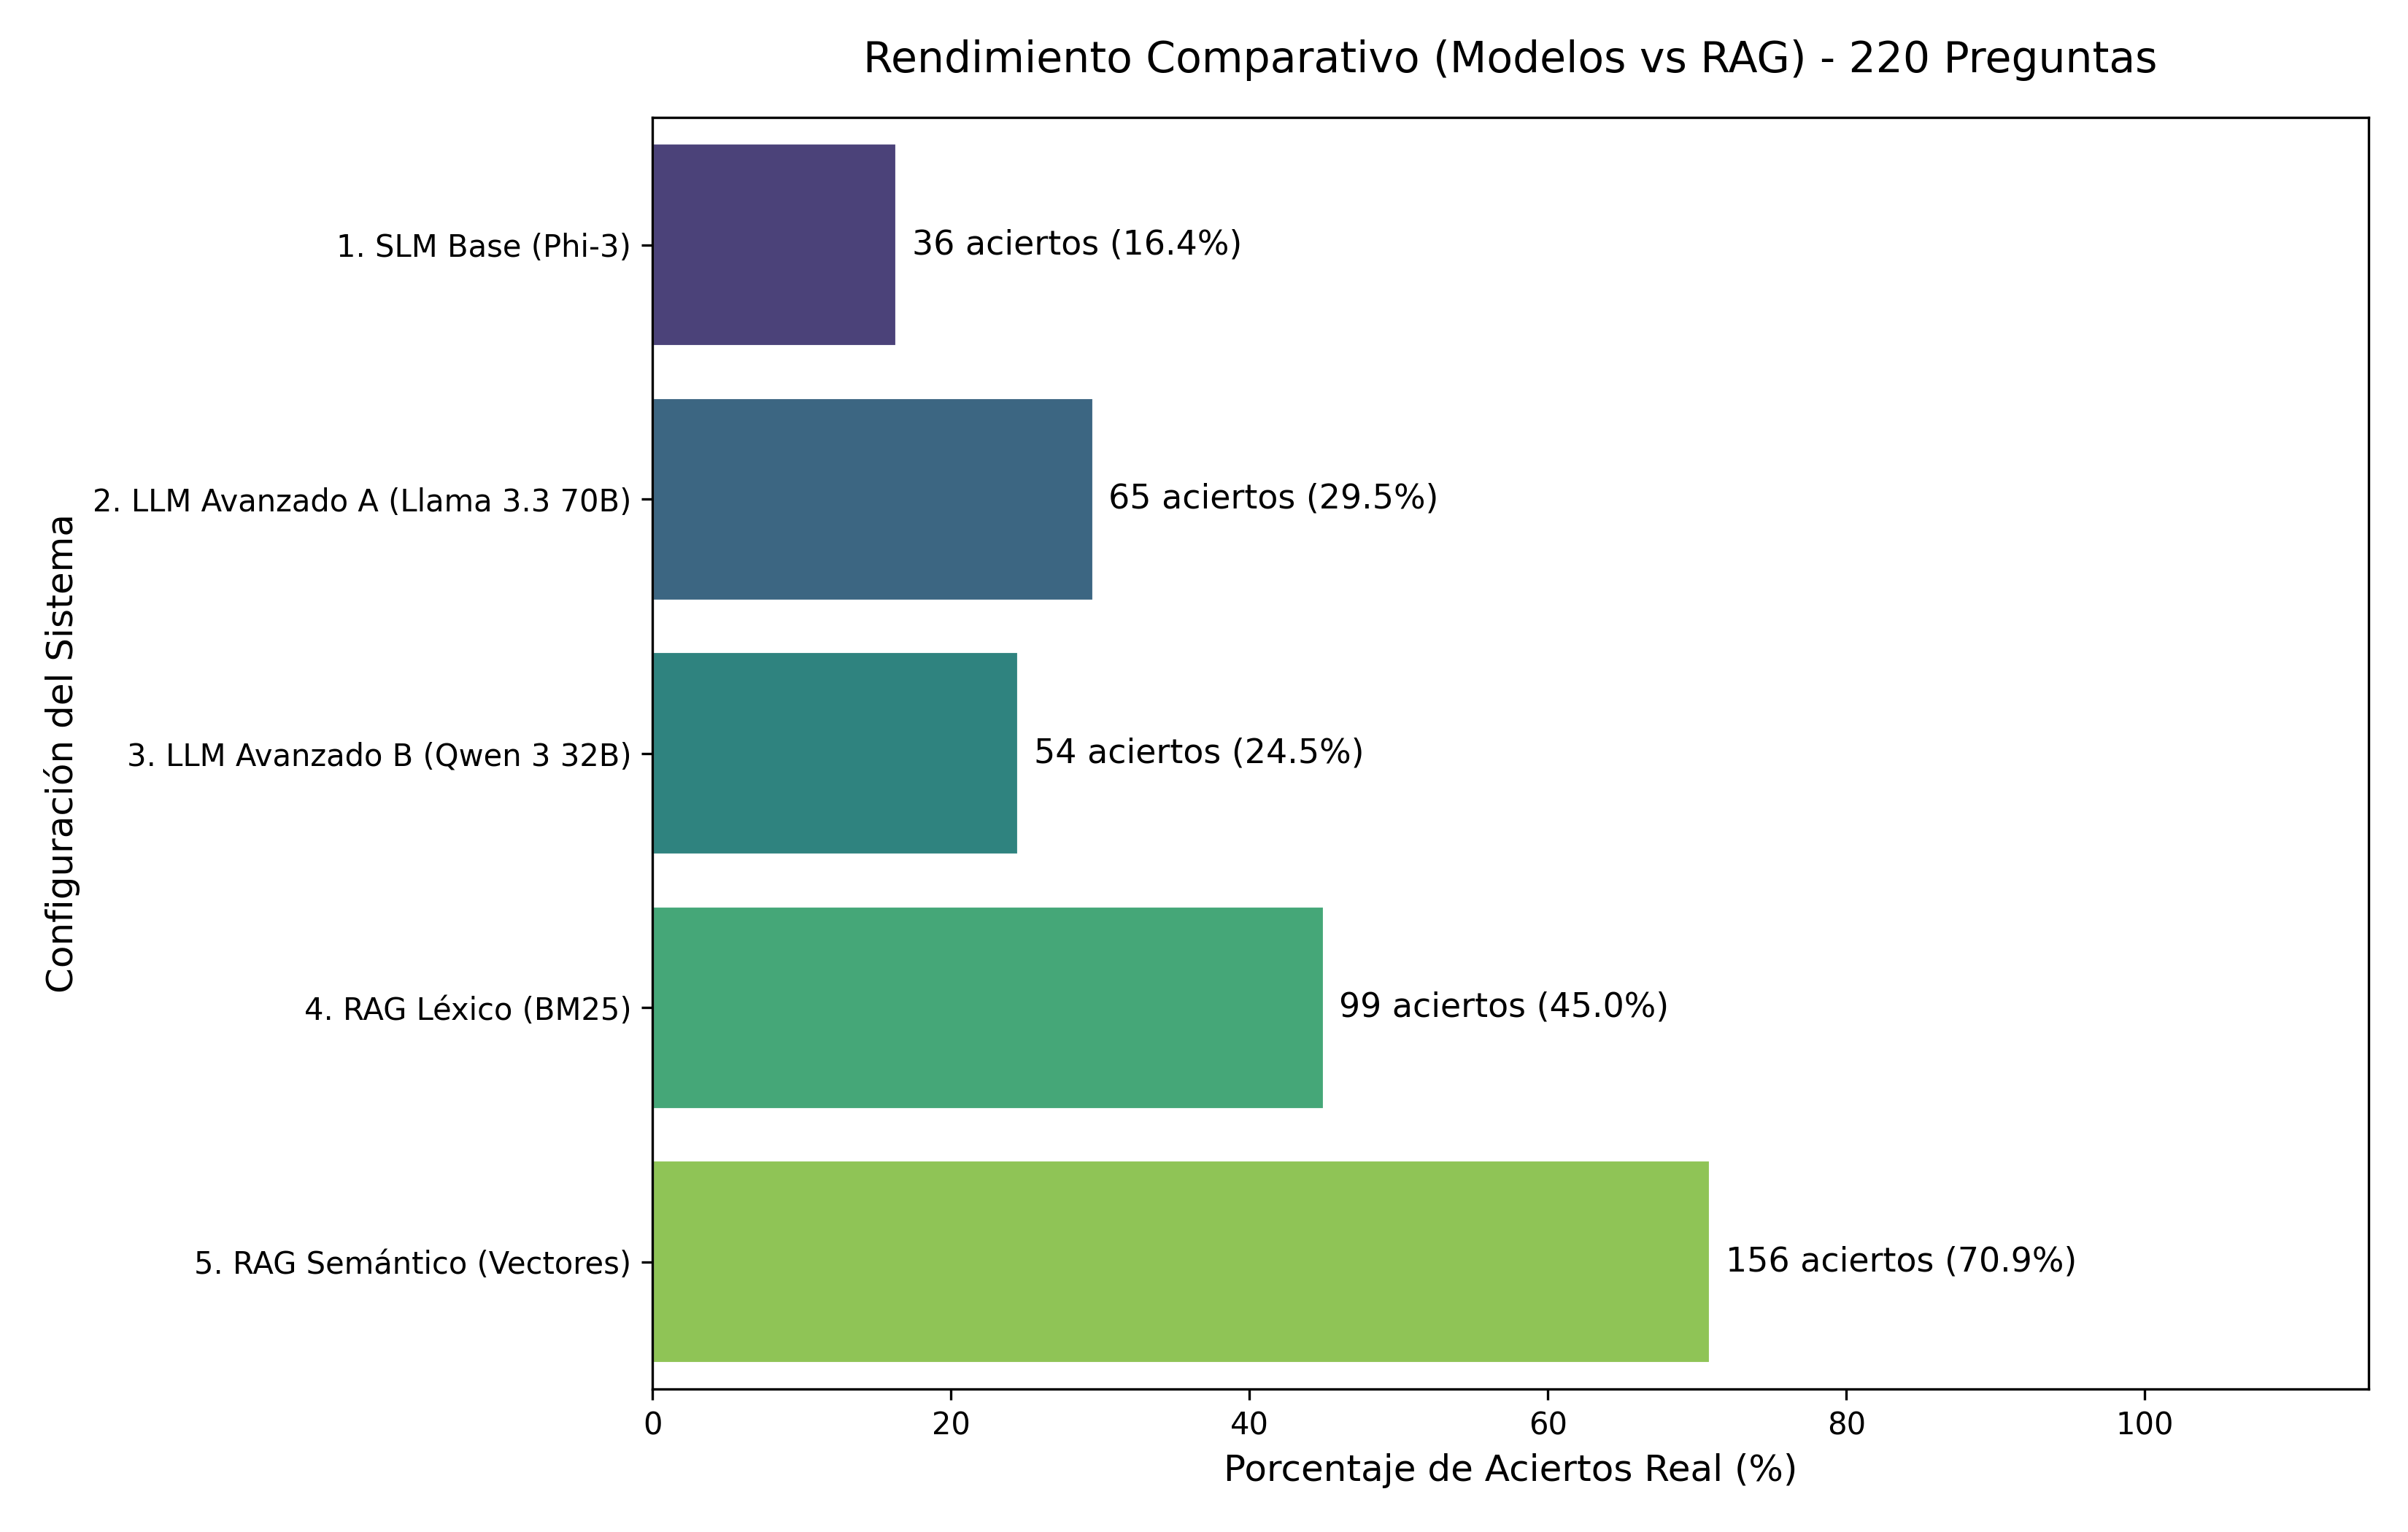
\includegraphics[width=0.95\textwidth]{archivos/grafico_rendimiento_220_preguntas.png}
    \caption{Rendimiento global de las cinco configuraciones sobre el dataset completo (220 preguntas). Se evidencia la superioridad absoluta del RAG Semántico.}
    \label{fig:evaluacion_220}
\end{figure}

Como se observa en el gráfico, ninguno de los modelos operando de memoria (\textit{Zero-Shot}) logró alcanzar el 30\% de precisión, quedando Llama 3.3 70B en un 29,5\% (65 aciertos) y Qwen 3 32B en un 24,5\% (54 aciertos). Por el contrario, la inyección de contexto transformó radicalmente el rendimiento del modelo más pequeño (Phi-3). En cuanto a los dos tipos de métodos de recuperación, mientras que el RAG Léxico elevó el rendimiento al 45,0\% (99 aciertos), fue el \textbf{RAG Semántico vectorial} el que obtuvo mayor porcentaje de aciertos con un \textbf{70,9\% de precisión (156 aciertos)}. 

Estos resultados demuestran, en primer lugar, la robustez intrínseca que una arquitectura RAG aporta al sistema de verificación; incluso la implementación léxica más sencilla permite que un modelo ligero supere en precisión factual a modelos mucho más potentes operando de forma aislada. En segundo lugar, los datos confirman la superioridad crítica de la recuperación semántica frente a la léxica. Al procesar las consultas dentro de un espacio vectorial denso, el sistema es capaz de capturar la intención y el significado de la pregunta, logrando una localización de evidencias mucho más precisa que el simple conteo de términos coincidentes de los algoritmos tradicionales como es el caso de BM25.

No obstante, la comparación entre los resultados de la fase piloto (80 preguntas, 91,2\% de aciertos en RAG Semántico) y los del \textit{dataset} completo (220 preguntas, 70,9\%) refleja una caída significativa que no indica una degradación del sistema, sino que sucede por dos factores que alteraron la composición y dificultad del conjunto de evaluación.

El primero tiene que ver con la distribución de tipos de pregunta. Como muestra la Tabla~\ref{tab:distribucion_dataset}, las primeras 80 preguntas presentaban una proporción más alta de preguntas trampa (22,50\% frente al 15,71\% de las siguientes 140), categoría en la que el RAG Semántico obtiene mejor tasa de acierto (se detallará esto mas adelante). Trasladando la proporción de preguntas trampa de la fase piloto al lote adicional de 140 preguntas, De haber mantenido la misma proporción de trampa que en la fase piloto, el lote adicional habría contenido unas 31 preguntas de ese tipo en lugar de las 22 que tiene, lo que equivale a que aproximadamente 9 preguntas son factuales o de inferencia donde antes habrían sido trampa.

El segundo factor tiene que ver con la dificultad temática de las preguntas. La búsqueda de diversidad temática en el \textit{dataset} llevó a que los temas de las primeras preguntas fueran eventos de alto impacto mediático (aranceles, DANA, Eurocopa, Taylor Swift), noticias con una mayor presencia en el corpus que facilitan la recuperación semántica al aparecer con más frecuencia. A medida que se agotaban los temas más representados, las preguntas posteriores abordaron ámbitos más concretos como el túnel marítimo de Génova, fármacos en fase de estudio contra el Alzheimer, Neuralink de Elon Musk o noticias de la sonda Athena entre otros. Estas preguntas exigen que el recuperador localice información en documentos menos frecuentes dentro del corpus, lo que eleva la dificultad de una correcta recuperación.

Ambos factores combinados explican la bajada del porcentaje global y, al mismo tiempo, refuerzan la validez del \textit{dataset} final como instrumento de evaluación más riguroso y representativo de escenarios reales de verificación factual.

\begin{table}[h]
\centering
\begin{tabular}{@{}lcccc@{}}
\toprule
\textbf{Tipo} & 
\textbf{Hasta preg. 80} & 
\textbf{\%} & 
\textbf{Desde preg. 81} & 
\textbf{\%} \\ \midrule
Factual    & 43 & 53,75\% & 100 & 71,43\% \\
Trampa     & 18 & 22,50\% & 22  & 15,71\% \\
Inferencia & 19 & 23,75\% & 18  & 12,86\% \\
\midrule
\textbf{Total} & \textbf{80} & \textbf{100\%} & 
\textbf{140} & \textbf{100\%} \\
\bottomrule
\end{tabular}
\caption{Distribución por tipo de pregunta entre la fase piloto y el lote adicional, mostrando el desplazamiento hacia preguntas factuales en la segunda fase.}
\label{tab:distribucion_dataset}
\end{table}
\newpage
\section{Análisis de Errores y Calidad del Sistema}

Más allá de las métricas cuantitativas globales, he decidido realizar un análisis cualitativo exhaustivo. En esta sección se analizan tanto la calidad de algunos casos puntuales como el desempeño del sistema ante diferentes tipologías de pregunta.

\subsection{Clasificación Cualitativa de Fallos}

Para ilustrar el impacto real de la arquitectura RAG frente a los modelos operando en \textit{Zero-Shot}, se han aislado cuatro casos de estudio representativos extraídos de la evaluación del \textit{dataset}. Estos ejemplos evidencian las fortalezas de la inyección de contexto, pero también exponen algunos ejemplos de vulnerabilidades del sistema.

\vspace{0.3cm}
\noindent\textbf{Caso 1: La alucinación factual frente a la evidencia recuperada} \\
Este caso demuestra el problema de la degradación temporal de los LLMs. Ante un dato numérico específico y reciente, el modelo masivo recurre a información desactualizada o alucinada, mientras que el RAG extrae el dato exacto del contexto.
\begin{table}[h]
\centering
\resizebox{\textwidth}{!}{%
\begin{tabular}{|p{3cm}|p{12cm}|}
\hline
\textbf{Pregunta} & ¿A cuánto llegó a subir Trump los aranceles a China? \\ \hline
\textbf{Esperada} & 145\% \\ \hline
\textbf{Llama 3.3 70B (Base)} & \textcolor{Maroon}{\textbf{Hasta un 25\% en algunos productos.}} \\ \hline
\textbf{Phi-3 (RAG Sem.)} & \textcolor{ForestGreen}{\textbf{Los aranceles a China llegan a subir hasta el 145\%.}} \\ \hline
\end{tabular}%
}
\end{table}

\noindent\textbf{Caso 2: La pregunta trampa y la capacidad de abstención} \\
Las preguntas sobre eventos no ocurridos o no reportados son el mayor caso de alucinación para los modelos (\textit{Zero-Shot}). Llama 3.3 70B intenta complacer al usuario inventando una respuesta, mientras que el RAG cumple estrictamente la instrucción de no inventar respuestas de su \textit{System Prompt}.
\begin{table}[h]
\centering
\resizebox{\textwidth}{!}{%
\begin{tabular}{|p{3cm}|p{12cm}|}
\hline
\textbf{Pregunta} & Tras el partido en el que la España de las finales vuelve a ganar la Liga de Naciones, ¿qué entrenadora alemana fue destituida de su cargo? \\ \hline
\textbf{Esperada} & No tengo información suficiente en mis archivos. \\ \hline
\textbf{Llama 3.3 70B (Base)} & \textcolor{Maroon}{\textbf{Martina Voss-Tecklenburg.}} \\ \hline
\textbf{Phi-3 (RAG Sem.)} & \textcolor{ForestGreen}{\textbf{No se proporciona información sobre la destitución de una entrenadora alemana en las noticias proporcionadas.}} \\ \hline
\end{tabular}%
}
\end{table}

\noindent\textbf{Caso 3: La anomalía del modelo ligero (Acierto Zero-Shot)} \\
Aunque poco frecuente, existen escenarios donde el conocimiento general encapsulado en un modelo pequeño (Phi-3) se alinea correctamente con la realidad, mientras que el modelo de mayor escala (Llama 3.3 70B) asume una premisa falsa.
\begin{table}[h]
\centering
\resizebox{\textwidth}{!}{%
\begin{tabular}{|p{3cm}|p{12cm}|}
\hline
\textbf{Pregunta} & Atendiendo a las características de la versión europea de Meta AI, ¿utilizó la empresa los datos de los internautas europeos para entrenar a su asistente virtual? \\ \hline
\textbf{Esperada} & No, Meta AI no se entrenó con datos de usuarios europeos. \\ \hline
\textbf{Llama 3.3 70B (Base)} & \textcolor{Maroon}{\textbf{Sí, Meta utilizó datos de internautas europeos para entrenar a su asistente virtual.}} \\ \hline
\textbf{Phi-3 (Base)} & \textcolor{ForestGreen}{\textbf{No, Meta AI no utiliza datos de internautas europeos para entrenar a su asistente virtual.}} \\ \hline
\end{tabular}%
}
\end{table}

\noindent\textbf{Caso 4: El fallo de recuperación} \\
El sistema RAG no es infalible. Si el motor de búsqueda (ya sea léxico o semántico) fracasa al recuperar el documento que contiene la respuesta, el modelo está forzado a abstenerse debido a su \textit{System Prompt} (aunque tenga conocimiento del tema). En este caso, la restricción del RAG juega en su contra frente a los modelos base, que sí conocían el dato cinematográfico en su memoria interna.
\begin{table}[h]
\centering
\resizebox{\textwidth}{!}{%
\begin{tabular}{|p{3cm}|p{12cm}|}
\hline
\textbf{Pregunta} & ¿Qué actor protagoniza la película 'On the Waterfront' (1953) mencionada en el artículo de los Óscar? \\ \hline
\textbf{Esperada} & Marlon Brando \\ \hline
\textbf{RAG (Ambos)} & \textcolor{Maroon}{\textbf{No tengo información suficiente en mis archivos.}} \\ \hline
\textbf{Modelos Base} & \textcolor{ForestGreen}{\textbf{Marlon Brando}} \\ \hline
\end{tabular}%
}
\end{table}

\noindent\textbf{Caso 5: Fallo de RAG por error tipográfico} \\
Debido a su dependencia del contexto, el sistema prioriza errores presentes en documentos recuperados frente a su conocimiento interno. Así, aunque los modelos base aciertan, el RAG Semántico reproduce el fallo de una noticia de octubre de 2025 con un error tipográfico evidente: \textit{"Cuando en 2026 Elon Musk funda Neuralink..."}
\begin{table}[h]
\centering
\resizebox{\textwidth}{!}{%
\begin{tabular}{|p{3cm}|p{12cm}|}
\hline
\textbf{Pregunta} & Según la historia estratégica detallada en el artículo, ¿en qué año fundó Elon Musk la compañía Neuralink? \\ \hline
\textbf{Esperada} & 2016 \\ \hline
\textbf{RAG Sem.} & \textcolor{Maroon}{\textbf{Elon Musk fundó la compañía Neuralink en el año 2026.}} \\ \hline
\textbf{Modelos Base} & \textcolor{ForestGreen}{\textbf{2026}} \\ \hline
\end{tabular}%
}
\end{table}

Estos casos evidencian que el sistema RAG es altamente efectivo para evitar alucinaciones. Sin embargo, su rendimiento final queda totalmente condicionado la precisión de la recuperación y la veracidad del contexto recuperado.

\subsection{Comparativa de Rendimiento según el Tipo de Pregunta}

Para evaluar la versatilidad del sistema, se desglosó el rendimiento en tres ejes fundamentales: preguntas factuales (143), de inferencia (37) y trampa (40). El análisis conjunto de estas dimensiones permite visualizar de forma integral los puntos fuertes y las carencias de cada configuración, tal y como se representa en la Figura~\ref{fig:radar_tipologia}.

\begin{figure}[h]
    \centering
    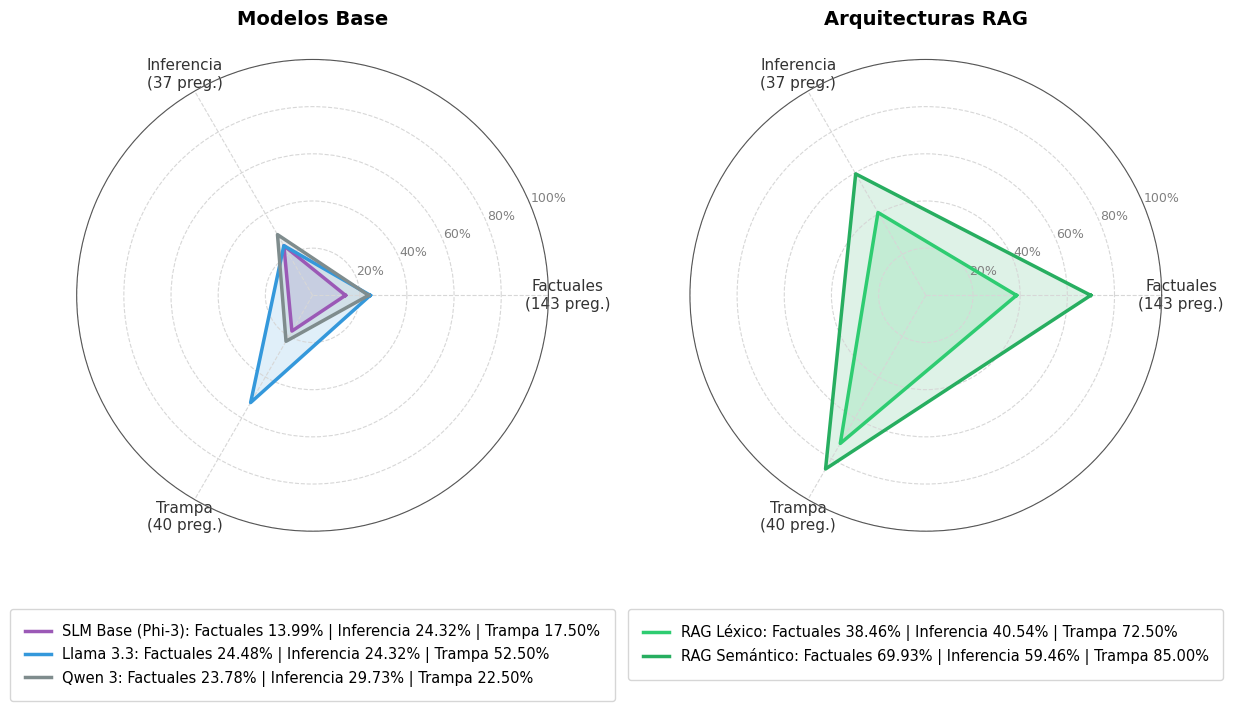
\includegraphics[width=\textwidth]{archivos/grafico_radar_doble.png}
    \caption{Comparativa de rendimiento por tipo de pregunta entre configuraciones.}
    \label{fig:radar_tipologia}
\end{figure}

La gráfica muestra claramente una brecha significativa de rendimiento entre operar exclusivamente con la memoria interna del modelo frente a la inyección de contexto externo. En el subgráfico de los modelos base, la representación visual muestra un área de rendimiento mínima que se mantiene en el centro del radar. Ninguno de los tres modelos logra superar el 30\% en preguntas factuales o de inferencia. Resulta especialmente crítico el comportamiento ante las preguntas trampa: Llama 3.3 70B destaca al lograr abstenerse en un 52,50\% de los casos, demostrando una mayor robustez ante la incertidumbre. En contraste, Phi-3 y Qwen 3 32B caen por debajo del 23\%, lo que puede representar un riesgo significativo de alucinación.

Por el contrario, el subgráfico de las arquitecturas RAG ilustra cómo la incorporación de contexto externo incrementa de forma notable el rendimiento global del sistema, destacando dos aspectos fundamentales de su comportamiento:

\begin{itemize}
    \item \textbf{Preguntas Factuales y de Inferencia:} Aunque la mejora ya es evidente con la recuperación léxica, los resultados más destacados se obtienen con el RAG semántico, que alcanza un 69,93\% y un 59,46\% de precisión, respectivamente. Estos datos confirman que el modelo de vectorización (BGE-M3) localiza eficazmente la información pertinente dentro del corpus de noticias.
    \item \textbf{Capacidad de Abstención (Preguntas Trampa):} Es en esta categoría donde ambos RAG sobresalen de manera excepcional. Tanto el enfoque léxico (72,50\% de acierto) como el semántico (85,00\%) demuestran una alta eficacia para identificar cuándo el contexto recuperado es insuficiente gracias a su \textit{System Prompt}, reduciendo drásticamente la generación de información inventada en comparación con los modelos base.
\end{itemize}

En conclusión, la adopción de esta arquitectura RAG implica un compromiso técnico claro: la mayoría de veces el sistema renuncia a responder basándose en el conocimiento externo del modelo (lo que explica fallos como el del Caso 4 que se comentaba previamente), pasando a depender por completo de la información extraída de las noticias. En el ámbito del \textit{Fact-Checking}, esta limitación es en realidad su mayor fortaleza, ya que garantiza que la respuesta emitida esté fundamentada en una fuente real, priorizando la fiabilidad por encima de la tasa de respuesta.
\newpage
\section{Discusión y Ensamblaje del Sistema Óptimo}

Una vez analizado el comportamiento de los modelos operando en solitario y evaluado el impacto de las diferentes estrategias de recuperación con un modelo ligero, el último paso de la investigación consiste en integrar los componentes más robustos para ensamblar la arquitectura definitiva con los componentes que mejores resultados han dado.

\subsection{El balance entre escala de modelo y precisión}
\label{sec:balance_escala}
La elección del modelo generador ideal para una arquitectura RAG no debe basarse únicamente en su capacidad para acertar preguntas, sino en su comportamiento ante la falta de información. Durante la fase de evaluación \textit{Zero-Shot}, los resultados demostraron que Llama 3.3 70B no solo fue el modelo con mayor tasa general de aciertos (29,5\%), sino que exhibió una superioridad crítica en la gestión de la incertidumbre.

Como se analizó previamente, ante las preguntas trampa, los modelos Phi-3 y Qwen 3 32B apenas lograron superar el 22\% de precisión, mostrando una alta propensión a inventar respuestas. Por el contrario, Llama 3.3 70B alcanzó un 52,5\% de éxito en esta misma categoría. Esta métrica resulta de vital importancia para el diseño del sistema final: un modelo base que ya posee un alto grado de alineación y sabe abstenerse de forma natural (\textit{Zero-Shot}) será estructuralmente más seguro al integrarse en un sistema RAG, ya que respetará de manera más estricta nuestras instrucciones cuando el motor de búsqueda no recupere información relevante  ya sea por un fallo del recuperador o porque no exista esa información en nuestra base de datos.

El tamaño del modelo influye directamente en su capacidad para seguir las restricciones del \textit{prompt} cuando estas contradicen su conocimiento interno. Mientras que los modelos pequeños (SLM) suelen presentar una mayor ``atracción semántica'' hacia su conocimiento interno (fenómeno que provoca que el modelo ignore las restricciones del \textit{prompt} si detecta conceptos familiares en sus pesos), Llama 3.3 70B permite una distinción nítida entre la memoria paramétrica y el contexto inyectado. En el marco del \textit{Fact-Checking}, esto se traduce en una reducción drástica de la ``creatividad'' estadística del modelo, haciendo que este se abstenga antes de generar contenido infundado.

\subsection{Arquitectura del Sistema RAG Final}

Teniendo en cuenta todo lo analizado anteriormente, se propone como solución óptima la combinación del modelo generador \textbf{Llama 3.3 70B} con el motor de recuperación \textbf{Semántico (BGE-M3)}. 

Esta selección conjunta no responde a una simple agregación de los componentes con mejores métricas individuales, sino a la necesidad de establecer un sistema de doble validación. En el dominio del \textit{Fact-Checking}, el coste de un falso positivo (dar por cierta una afirmación falsa o inventar un dato) es inasumible. Por un lado, BGE-M3 asume el rol de maximizar la ingesta de contexto relevante, minimizando los puntos ciegos de la búsqueda léxica. Por otro, al delegar la síntesis a un modelo masivo como Llama 3.3 70B, se instaura un mecanismo de contingencia crítico: si la recuperación resulta infructuosa o el texto extraído es ambiguo, el generador se abstiene en lugar de forzar una respuesta o dejarse sesgar por un contexto deficiente, asegurando que el proceso culmine en una abstención segura. Por tanto, con esta arquitectura no se busca simplemente aumentar la tasa de aciertos, sino también que los fallos cometidos sean preferiblemente falsos negativos (abstenciones) en lugar de falsos positivos (alucinaciones).

Para validar esta arquitectura final, se ejecutó una evaluación del \textit{dataset} completo (220 preguntas). Los resultados globales se consolidan en la Figura~\ref{fig:comparativa_global}.

\begin{figure}[h]
    \centering
    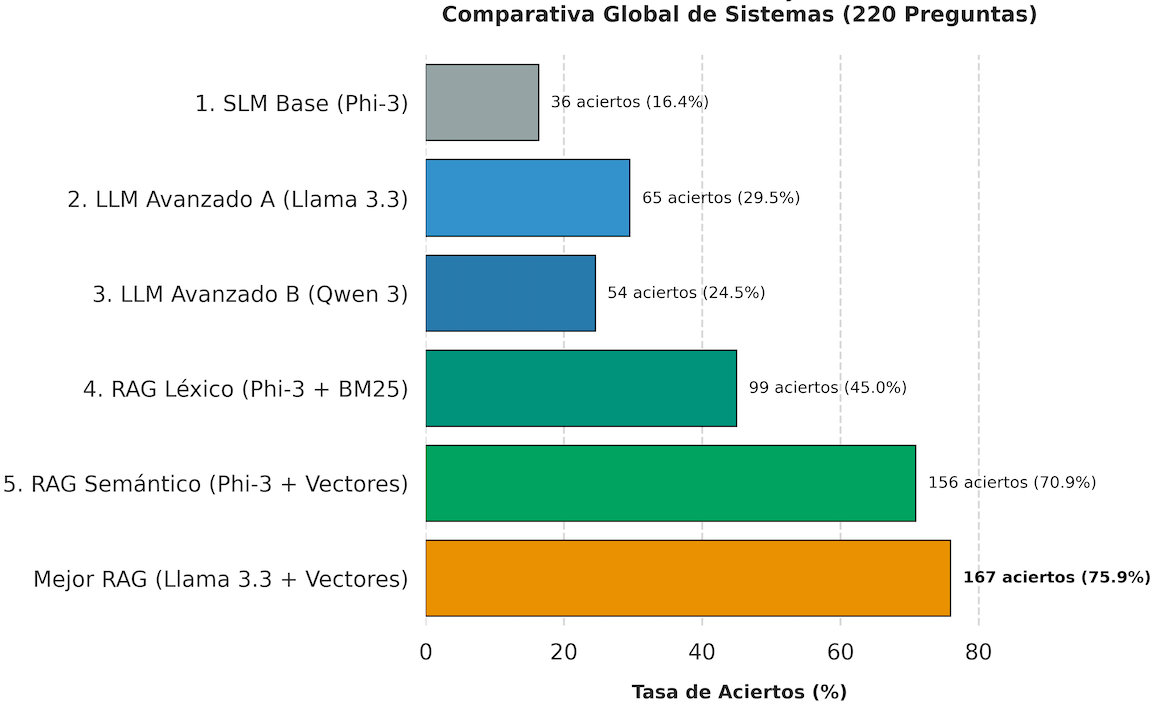
\includegraphics[width=\textwidth]{archivos/grafico_barras_final.png}
    \caption{Comparativa de la tasa de aciertos entre los modelos base, las arquitecturas RAG con SLM (Phi-3) y el sistema RAG óptimo (Llama 3.3 70B + Vectores).}
    \label{fig:comparativa_global}
\end{figure}
Como ilustra la gráfica, el sistema RAG Óptimo obtiene el nuevo mejor resultado de la investigación con un \textbf{75,9\% de precisión (167 aciertos)}. Al comparar este incremento con el obtenido por el RAG Semántico de Phi-3 (156 aciertos), confirmamos que la mejora de resultados más drástica se logra mediante la implementación y perfeccionamiento del motor de recuperación (de Zero-Shot a RAG, y de BM25 a Vectores), mucho más que por el cambio de modelo generador. No obstante, utilizar un modelo más grande sigue siendo una pieza fundamental que aporta un margen de mejora adicional y muy significativo al sistema.

Para ofrecer una visión integral del progreso acumulado a lo largo de toda la investigación, la Tabla~\ref{tab:resumen_global} consolida en un único lugar el rendimiento de las seis configuraciones evaluadas, desglosado por tipo de pregunta sobre el \textit{dataset} completo de 220 preguntas.

\begin{table}[ht]
\centering
\resizebox{\textwidth}{!}{%
\begin{tabular}{@{}lcccccccc@{}}
\toprule
\multirow{2}{*}{\textbf{Configuración}} &
\multicolumn{2}{c}{\textbf{Factuales (143)}} &
\multicolumn{2}{c}{\textbf{Inferencia (37)}} &
\multicolumn{2}{c}{\textbf{Trampa (40)}} &
\multicolumn{2}{c}{\textbf{Total (220)}} \\
\cmidrule(lr){2-3} \cmidrule(lr){4-5} \cmidrule(lr){6-7} \cmidrule(lr){8-9}
& \textbf{Aciertos} & \textbf{\%} & \textbf{Aciertos} & \textbf{\%}
& \textbf{Aciertos} & \textbf{\%} & \textbf{Aciertos} & \textbf{\%} \\
\midrule
1. SLM Base (Phi-3)                    & 20  & 14,0\% & 9  & 24,3\% & 7  & 17,5\% & 36  & 16,4\% \\
2. LLM Avanzado A (Llama 3.3 70B)          & 35  & 24,5\% & 9  & 24,3\% & 21 & 52,5\% & 65  & 29,5\% \\
3. LLM Alternativo (Qwen 3 32B)            & 34  & 23,8\% & 11 & 29,7\% & 9  & 22,5\% & 54  & 24,5\% \\
4. RAG Léxico (Phi-3 + BM25)           & 55  & 38,5\% & 15 & 40,5\% & 29 & 72,5\% & 99  & 45,0\% \\
5. RAG Semántico (Phi-3 + BGE-M3)      & 100 & 69,9\% & 22 & 59,5\% & 34 & 85,0\% & 156 & 70,9\% \\
6. RAG Óptimo (Llama 3.3 70B + BGE-M3)    & 103 & 72,0\% & 25 & 67,6\% & 38 & 95,0\% & 167 & 75,9\% \\
\bottomrule
\end{tabular}%
}
\caption{Resumen consolidado del rendimiento de todas las configuraciones evaluadas, desglosado por tipo de pregunta sobre el \textit{dataset} completo de 220 preguntas.}
\label{tab:resumen_global}
\end{table}

La tabla permite leer de forma conjunta las dos narrativas principales del trabajo. En sentido horizontal, se aprecia cómo cada configuración responde de manera diferenciada a cada tipología: las preguntas trampa, que exigen abstención, son las que mayor varianza presentan entre sistemas, desde el 17,5\% de Phi-3 en estado base hasta el 95,0\% del sistema óptimo. En sentido vertical, la tabla cuantifica el salto acumulado que supone cada decisión de diseño: pasar de Zero-Shot a RAG Léxico ya aporta entre 15 y 55 puntos porcentuales según la categoría, mientras que el salto adicional al RAG Semántico resulta de nuevo más determinante que el cambio de generador.

Precisamente este último dato, la mejora de 3 puntos en factuales y 8 puntos en inferencia al sustituir Phi-3 por Llama 3.3 70B manteniendo el mismo recuperador, ilustra que el techo del sistema lo fija la calidad de la recuperación, y que el modelo generador actúa como un amplificador de aquello que el motor de búsqueda es capaz de encontrar.

\subsection{Análisis de Errores: El Impacto del Modelo Generador}

Más allá de evaluar el incremento de 5 puntos porcentuales en la precisión global (del 70,9\% al 75,9\%), el siguiente paso en la evaluación consiste en comprobar qué tipo de errores cometen estos sistemas y cómo se distribuyen. Para llevar a cabo este análisis, se ha clasificado el comportamiento de ambas arquitecturas RAG Semánticas en tres categorías clave:

\begin{itemize}
    \item \textbf{Abstención (Negativa Correcta):} Preguntas trampa en las que el modelo indicó correctamente que no tenía información suficiente en el contexto para responder (clasificadas como acierto).
    \item \textbf{No Alucinación:} Preguntas que sí tenían una respuesta concreta, pero el modelo falló al extraerla o no la encontró. Sin embargo, supo abstenerse de forma segura en lugar de inventar el dato (clasificadas como fallo, pero seguro).
    \item \textbf{Alucinación:} Preguntas en las que el modelo se equivocó al no abstenerse, aportando una respuesta inventada o errónea. Esta categoría agrupa tanto los errores factuales (extracción incorrecta de información presente en el contexto) como las alucinaciones propiamente dichas (generación de contenido no respaldado por el contexto).
\end{itemize}

Cabe destacar que, para centrar el análisis exclusivamente en el analisis de errores y la capacidad de abstención, se ha tomado la decisión de excluir de esta comparativa los aciertos simples de preguntas factuales o de inferencia.

\begin{figure}[h]
    \centering
    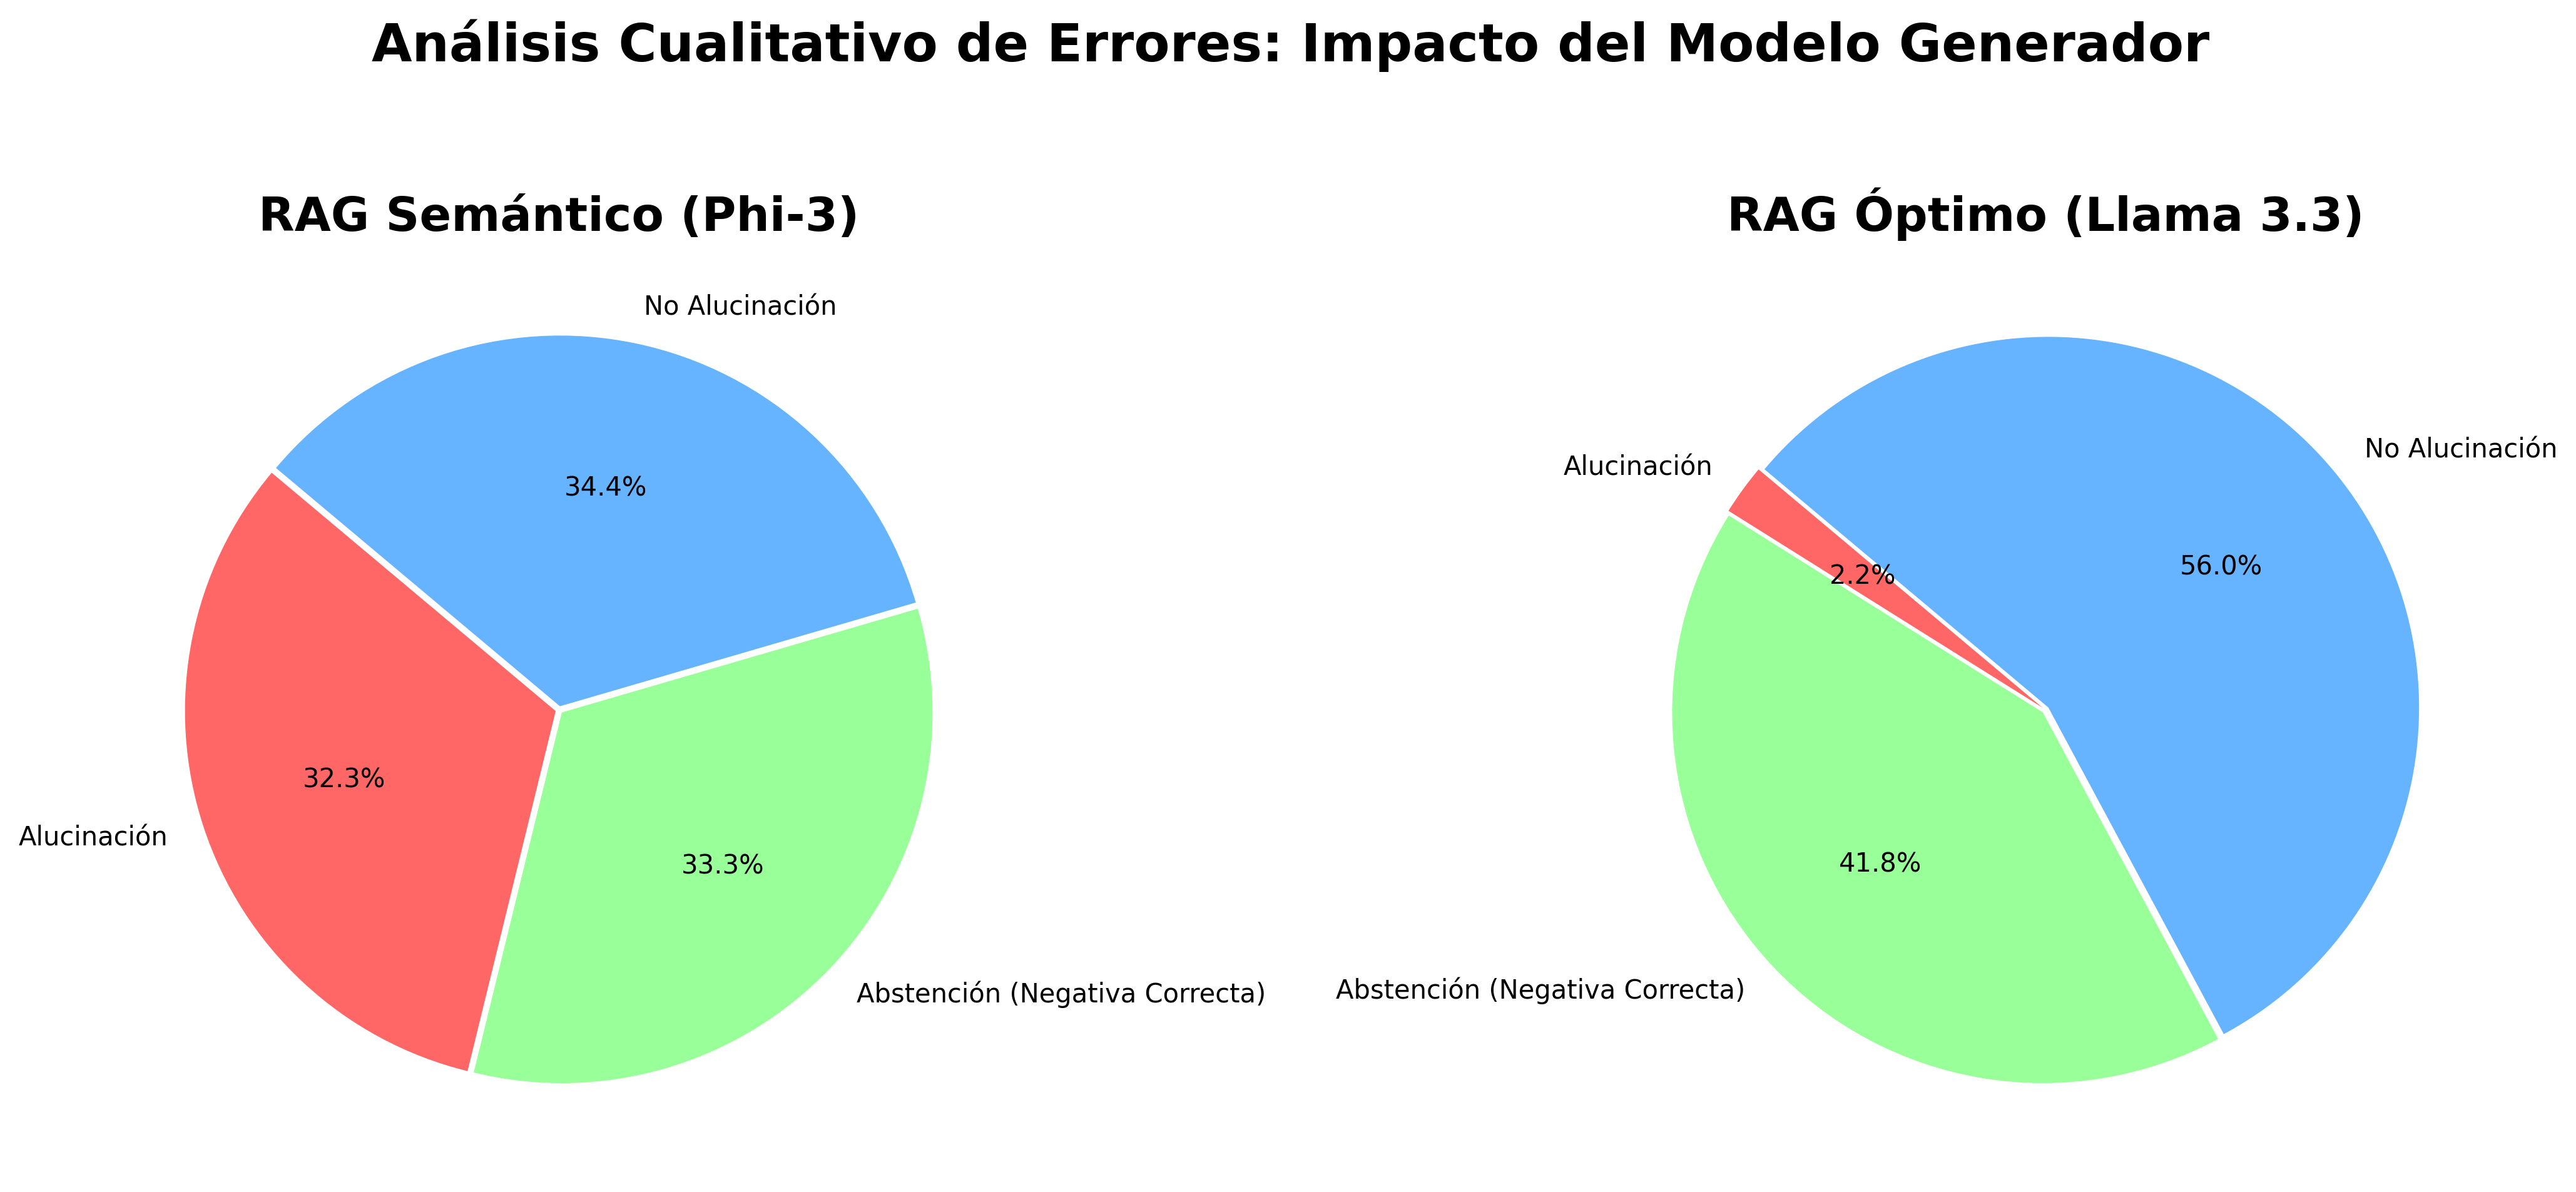
\includegraphics[width=\textwidth]{archivos/grafico_sectores_errores.png}
    \caption{Comparativa cualitativa de errores. Se evidencia la drástica reducción de la tasa de alucinación al emplear un modelo base con mayor grado de alineación.}
    \label{fig:analisis_errores}
\end{figure}

El análisis expuesto en la Figura~\ref{fig:analisis_errores} revela un aspecto fundamental del comportamiento de ambos sistemas. Aunque la diferencia en la tasa de aciertos entre el RAG Semántico con Phi-3 y el RAG Óptimo con Llama 3.3 70B no haya sido super significativa (5\% de aumento), es en la distribución de errores donde se observa un cambio realmente notable. Más allá de acertar un mayor número de preguntas, el verdadero logro de Llama 3.3 70B radica en haber conseguido reducir de forma drástica el porcentaje de alucinaciones ante la falta de información pertinente.

Este comportamiento respalda directamente la premisa detallada en el epígrafe \ref{sec:balance_escala}: Como se observó en la evaluación de los modelos base sin RAG, Llama 3.3 70B ya superaba ampliamente a los otros dos modelos en su capacidad de abstención; esta cualidad intrínseca ha demostrado ser estructuralmente mucho más eficaz al trasladarla a una arquitectura RAG Semántica, mejorando de forma evidente la fiabilidad que teníamos en la mejor arquitectura anterior. Tomando como denominador el total de casos no resueltos correctamente por cada sistema (es decir, excluyendo los aciertos directos), Phi-3 generó alucinaciones en un \textbf{32,3\%} de dichos casos, evidenciando las limitaciones del SLM para seguir instrucciones estrictas. Llama 3.3 70B reduce estos fallos a un \textbf{2,2\%} sobre el mismo denominador.

Al trasladar su superioridad paramétrica al entorno RAG, se observa que Llama 3.3 70B no solo domina las negativas correctas (\textbf{41,8\%}) (vital ya que demuestra la capacidad del sistema para detectar preguntas trampa), sino que altera por completo la naturaleza de los errores que comete. Cuando se enfrenta a una pregunta de la que no logra obtener el contexto adecuado para responder, se abstiene de forma segura en el \textbf{56,0\%} de los casos (\textit{No Alucinación}). En definitiva, el uso de este LLM erradica prácticamente el riesgo de desinformación, transformando las alucinaciones peligrosas en abstenciones y culminando en un marco de \textit{Fact-Checking} mucho más confiable.

